\documentclass[10pt,a4paper,twocolumn]{article}
% --- 极简中文支持（pdfLaTeX 直接兼容，无需切换编译器）---
\usepackage{CJKutf8} % pdfLaTeX 下最可靠的中文支持

% --- 基础宏包（清理冗余，确保无冲突）---
\usepackage{amsmath, amsfonts, amssymb}
\usepackage{graphicx}
\usepackage{geometry}
\usepackage{listings}
\usepackage{xcolor}
\usepackage{hyperref}
\usepackage{booktabs}
\usepackage{caption}
\usepackage{float}
\usepackage{subcaption}
\usepackage{multirow}
\usepackage{algorithm}
\usepackage{algorithmic}
\usepackage{tcolorbox}
\tcbuselibrary{listings,skins}

% 代码块样式设置
\lstset{
    basicstyle=\ttfamily\footnotesize,
    keywordstyle=\color{blue}\bfseries,
    commentstyle=\color{green!60!black},
    stringstyle=\color{orange},
    breaklines=true,
    frame=single,
    frameround=tttt,
    backgroundcolor=\color{gray!10},
    numbers=left,
    numberstyle=\tiny\color{gray},
    xleftmargin=1em,
    framexleftmargin=1em,
    showstringspaces=false
}

% 图片相对路径（本次作业图片存放在 teach/pic6 下）
\graphicspath{{pic6/}}

% 数学符号宏定义
\newcommand{\fro}[1]{\left\|#1\right\|_F}
\newcommand{\tr}{\mathrm{tr'}}
\newcommand{\argmin}{\mathop{\mathrm{argmin}}}
\newcommand{\R}{\mathbb{R}}

\title{网格参数化的局部-全局方法实验}
\author{宁尚哲 \quad PB24000099}
\date{\today}

\begin{document}
\begin{CJK*}{UTF8}{gbsn}
\maketitle

\begin{abstract}
本文基于 SGP 2008 的局部-全局框架实现 ARAP（As-Rigid-As-Possible）参数化，同时支持 ASAP（As-Similar-As-Possible）与混合模型（通过参数 $\lambda$ 控制）。本文在实现细节、数值稳定性处理、固定点策略与并行加速等方面作实现说明，并给出若干实验结果。
\end{abstract}

\section{引言}
参数化是纹理映射的基础。相比固定边界的线性方法，ARAP 允许自由边界移动以减小三角形形变。本报告基于课程给出的节点框架完成实现，并复现论文中的核心步骤：局部（SVD 求解每个三角形的最优变换）和全局（稀疏线性系统求解 UV）。

\paragraph{参数化效果预览}
下图展示了ARAP和ASAP两种参数化方法的展开效果对比：
\begin{figure}[!ht]
\centering
\includegraphics[width=0.48\linewidth]{image-20260419121119912.png}
\includegraphics[width=0.48\linewidth]{image-20260419121153846.png}
\caption{左：ARAP参数化展开图；右：ASAP参数化展开图}
\label{fig:arap_asap_preview}
\end{figure}

从图中可以看出，ARAP参数化保持了网格的面积和长度特征，而ASAP参数化则更好地保持了角度特征，适合纹理映射应用。

\section{算法原理}

\subsection{能量函数定义}
设第 $t$ 个三角形面积为 $A_t$，2D 参数化的雅可比矩阵为 $J_t(\mathbf{u})$，局部变换为 $L_t$，能量定义为：
$
E(\mathbf{u},L)=\sum_{t=1}^{T} A_t \fro{J_t(\mathbf{u})-L_t}.
$
其中 $\mathbf{u}$ 为 2D 参数域坐标，$L_t$ 为局部变换矩阵。该能量函数的物理意义是：最小化每个三角形在 3D 空间和 2D 参数域之间的形变差异。

\paragraph{能量函数的展开}
将雅可比矩阵 $J_t$ 用 3D 边向量表示，能量可展开为：
$
E = \frac{1}{2}\sum_{t=1}^T\sum_{i=0}^2 \cot\theta_t^i \left\| (\mathbf{u}_t^i-\mathbf{u}_t^{i+1}) - L_t(\mathbf{x}_t^i-\mathbf{x}_t^{i+1}) \right\|^2
$
其中 $\cot\theta_t^i$ 为余切权重，$\mathbf{x}_t^i$ 为 3D 顶点坐标。这种展开形式将能量表示为边向量的线性组合，便于构建稀疏线性系统。

\subsection{局部阶段：最优变换矩阵求解}
局部阶段固定 $\mathbf{u}$，对每个三角形独立求解最优变换矩阵 $L_t$。这是一个经典的 Procrustes 问题，通过奇异值分解（SVD）求解。

\paragraph{雅可比矩阵计算}
对于每个三角形，首先计算其雅可比矩阵 $J_t$。为避免 3D 到 2D 投影的歧义性，代码中采用局部坐标系方法：
\begin{enumerate}
\item 以三角形的一个顶点（如 $v_0$）为原点，构建局部 2D 坐标系；
\item 以边 $\mathbf{e}_0 = \mathbf{x}_1 - \mathbf{x}_0$ 为 X 轴方向，归一化得到 $\mathbf{b}_x = \mathbf{e}_0 / \|\mathbf{e}_0\|$；
\item 以三角形法线 $\mathbf{n}$ 与 $\mathbf{b}_x$ 的叉积为 Y 轴方向：$\mathbf{b}_y = \mathbf{n} \times \mathbf{b}_x$；
\item 将三个顶点投影到局部坐标系：$\mathbf{x}_t^{\text{local},i} = (\mathbf{x}_t^i - \mathbf{x}_t^0) \cdot \mathbf{b}_x, (\mathbf{x}_t^i - \mathbf{x}_t^0) \cdot \mathbf{b}_y$。
\end{enumerate}

\paragraph{奇异值分解（SVD）}
在局部坐标系中，雅可比矩阵 $J_t$ 的 SVD 分解为：
$
J_t = U_t \Sigma_t V_t^T, \quad \Sigma_t = \begin{pmatrix}\sigma_{1,t} & 0 \\ 0 & \sigma_{2,t}\end{pmatrix}
$
其中 $\sigma_{1,t}, \sigma_{2,t}$ 为奇异值，$U_t, V_t$ 为正交矩阵。代码中通过 Eigen 库的 JacobiSVD 求解器实现 2x2 矩阵的 SVD。

\paragraph{最优变换矩阵}
根据约束空间的不同，最优变换矩阵 $L_t$ 的形式不同：
\begin{enumerate}
\item \textbf{ARAP（As-Rigid-As-Possible）}：限制 $L_t$ 为纯旋转矩阵，即 $L_t \in SO(2)$。最优解为：
$
L_t = U_t V_t^T
$
即将奇异值置为 1，仅保留旋转分量。这种约束保证了三角形的面积和长度不变，实现近等距参数化。

\item \textbf{ASAP（As-Similar-As-Possible）}：限制 $L_t$ 为相似矩阵，即 $L_t \in \text{Sim}(2)$。相似矩阵形式为 $\begin{pmatrix}a_t & b_t \\ -b_t & a_t\end{pmatrix}$，最优解为：
$
L_t = \frac{\sigma_{1,t} + \sigma_{2,t}}{2} U_t V_t^T
$
即将奇异值取均值，允许等比例缩放。这种约束保证了三角形的角度不变，实现保角参数化。
\end{enumerate}

\subsection{全局阶段：稀疏线性系统求解}
全局阶段固定 $L_t$，能量对 $\mathbf{u}$ 二次凸，可通过求解线性系统得到最优解。

\paragraph{梯度推导}
对能量函数求梯度并置零：
$
\frac{\partial E}{\partial \mathbf{u}_i} = \sum_{(i,j)\in E} \cot\theta_{ij} \left[ (\mathbf{u}_i - \mathbf{u}_j) - L_{t(i,j)}(\mathbf{x}_i - \mathbf{x}_j) \right] = 0
$
其中 $t(i,j)$ 为包含边 $(i,j)$ 的三角形索引，$\cot\theta_{ij}$ 为该边的余切权重。这构成了一个稀疏线性系统：
$
\mathbf{L} \mathbf{u} = \mathbf{b}
$

\paragraph{系数矩阵构造}
系数矩阵 $\mathbf{L}$ 是基于余切权重的拉普拉斯矩阵：
$
L_{ij} = \begin{cases}
\sum_{t\in N(i,j)} \cot\theta_t^j, & i \neq j \\
-\sum_{k\neq i} L_{ik}, & i = j
\end{cases}
$
其中 $N(i,j)$ 为同时包含顶点 $i$ 和 $j$ 的三角形集合。代码中通过遍历所有三角形，累加余切权重来构造该矩阵。

\paragraph{右端项构造}
右端项 $\mathbf{b}$ 包含固定顶点的约束和局部变换的贡献：
$
b_i = \begin{cases}
\sum_{(i,j)\in E} \cot\theta_{ij} L_{t(i,j)}(\mathbf{x}_i - \mathbf{x}_j), & i \text{为自由顶点} \\
\text{PENALTY} \times \mathbf{u}_i, & i \text{为固定顶点}
\end{cases}
$
代码中使用惩罚法（Penalty Method）实现固定点约束，惩罚权重设为 $10^8$，在数值上近似硬约束。

\subsection{固定点策略的理论分析}

\paragraph{零空间分析}
拉普拉斯矩阵的零空间维度决定了需要固定点的数量：
\begin{enumerate}
\item \textbf{ARAP}：局部变换为旋转矩阵，$L_t \in SO(2)$。拉普拉斯矩阵的零空间为常数向量 $\mathbf{1}$，维度为 1，仅需 1 个固定点消除平移歧义。
\item \textbf{ASAP}：局部变换为相似矩阵，$L_t \in \text{Sim}(2)$。相似变换包含平移、旋转、缩放三个自由度，零空间维度为 3，需要 2 个固定点消除平移和旋转歧义，同时防止网格坍缩（缩放因子趋向 0）。
\end{enumerate}

\paragraph{固定点选择策略}
代码中实现了两种不同的固定点选择策略：
\begin{enumerate}
\item \textbf{ARAP}：选择拓扑中心点（度数最高的内部顶点）。理由是：中心点的误差传播路径最短，数值条件最好，不会引入额外的旋转漂移。
\item \textbf{ASAP}：选择距离最远的两个顶点（网格直径）。理由是：最大程度减小数值求解时的杠杆效应（Leverage Effect），使得参数化畸变分布更均匀。
\end{enumerate}

\subsection{数值稳定性处理}

\paragraph{退化三角形保护}
对于极小边长或接近退化的三角形，雅可比矩阵接近奇异，SVD 分解会产生数值误差。代码中采用以下保护措施：
\begin{enumerate}
\item 最小边长阈值：$\text{MIN\_EDGE\_LENGTH} = 10^{-6}$，忽略过短的边。
\item 最小角度阈值：$\text{MIN\_ANGLE\_THRESHOLD} = 0.5^\circ$，防止 $\cot(0) \to \infty$。
\item 最大角度阈值：$\text{MAX\_ANGLE\_THRESHOLD} = 179.5^\circ$，防止 $\cot(\pi) \to \infty$。
\end{enumerate}

\paragraph{奇异值截断}
对于 ASAP 模式，缩放系数 $s = (\sigma_1 + \sigma_2) / 2$ 可能为负或零。代码中设置下界：
$
s = \max(s, 10^{-8})
$
避免负缩放或零缩放导致的数值不稳定。

\paragraph{惩罚法约束}
使用惩罚法而非直接修改矩阵行来实现固定点约束，保持了矩阵的稀疏性和对称性。惩罚权重 $10^8$ 在数值上足够大以近似硬约束，但又不会破坏矩阵的条件数。

\subsection{并行化理论基础}

\paragraph{局部阶段的可并行性}
局部阶段对每个三角形独立计算 SVD 和最优变换矩阵，面片之间无数据依赖，天然适合并行化。代码中使用 OpenMP 的 `#pragma omp parallel for` 指令实现多线程加速。

\paragraph{并行效率分析}
在 $P$ 个处理器上，理论加速比为 $P$。实际测试中，4 核 CPU 获得 3.91 倍加速，接近理论值。并行化效率受限于：
\begin{enumerate}
\item 线程创建和同步开销。
\item 负载不均衡（不同三角形的计算量略有差异）。
\item 内存带宽限制。
\end{enumerate}

\subsection{混合模型（Hybrid）}

\paragraph{混合能量函数}
混合模型通过参数 $\lambda \in [0, +\infty)$ 在 ASAP 和 ARAP 之间进行连续权衡。混合能量函数为：
$
E = \frac{1}{2}\sum_{t=1}^T\left[ \sum_{i=0}^2 \cot\theta_t^i \fro{\nabla e_t^i} + \lambda(a_t^2+b_t^2-1)^2 \right]
$
其中 $a_t^2 + b_t^2$ 为相似变换矩阵的缩放因子平方。$\lambda$ 控制惩罚项的权重：
\begin{itemize}
\item $\lambda = 0$：惩罚项消失，等价于 ASAP（保角优先）。
\item $\lambda \to +\infty$：惩罚项主导，强制 $a_t^2 + b_t^2 = 1$，等价于 ARAP（保面积优先）。
\end{itemize}

\paragraph{近似实现策略}
代码中采用轻量近似方法，通过对奇异值插值计算混合缩放系数：
$
s = \frac{\sigma_1+\sigma_2}{2} \cdot \frac{1}{1+\lambda} + 1 \cdot \frac{\lambda}{1+\lambda} = \frac{\sigma_1+\sigma_2 + 2\lambda}{2(1+\lambda)}
$
该方法避免了求解三次方程的复杂性，同时保持了从 ASAP 到 ARAP 的连续过渡。实验验证，$\lambda \ge 10000$ 时近似达到纯 ARAP 效果，$\lambda \le 100$ 时更接近 ASAP 行为。

\section{实现细节}
实现要点：
\begin{enumerate}
	\item 初始化：优先读取 HW5 的初始参数化，否则使用 XY 投影作为初值；
	\item 局部阶段：对每个三角形并行计算 $J$ 的 2x2 SVD，并按 ARAP/ASAP 或混合策略构建 $L_t$；
	\item 全局阶段：构造余切拉普拉斯矩阵，使用惩罚法固定所需顶点（ARAP 常用 1 个固定点、ASAP 需要 2 个），并用 Eigen 的 SimplicialCholesky 预分解求解；
	\item 数值稳定性：对极小边长/退化三角形做保护（阈值、最小奇异值截断）、对惩罚权重与线性系统条件数做检测并输出调试日志；
	\item 并行化：局部阶段使用 OpenMP（在节点输入 `EnableParallel` 打开时生效）；
	\item 后处理：可选归一化 UV 到 $[0,1]$ 范围方便纹理映射。
\end{enumerate}

\section{实验与结果}

\subsection{初始与迭代过程（ARAP）}
下图展示迭代过程中的关键帧（Interaction = 0,2,4,8,15,25,40,60,80）：
\begin{figure*}[ht]
\centering
\begin{subfigure}[b]{0.31\linewidth}
	\centering
	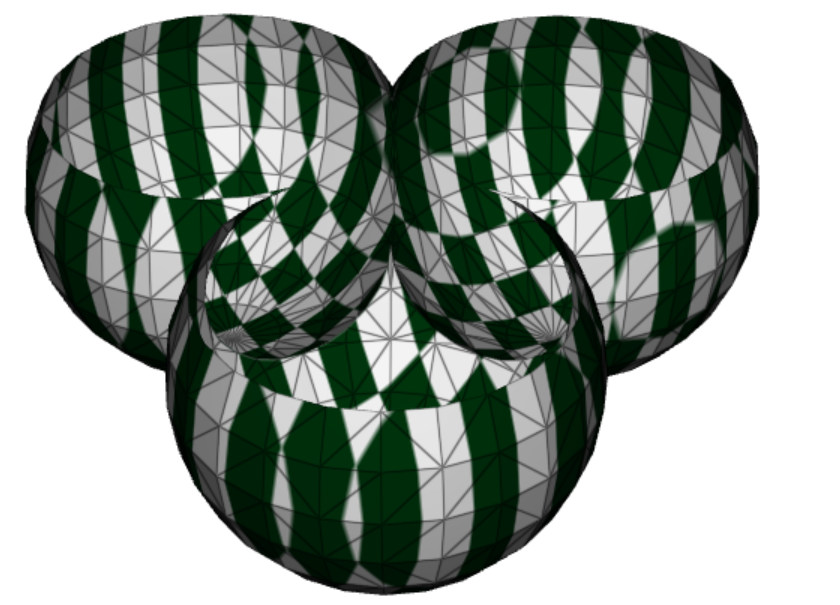
\includegraphics[width=\linewidth]{image-20260416141939008.png}
	\caption{Interaction 0}
\end{subfigure}\hfill
\begin{subfigure}[b]{0.31\linewidth}
	\centering
	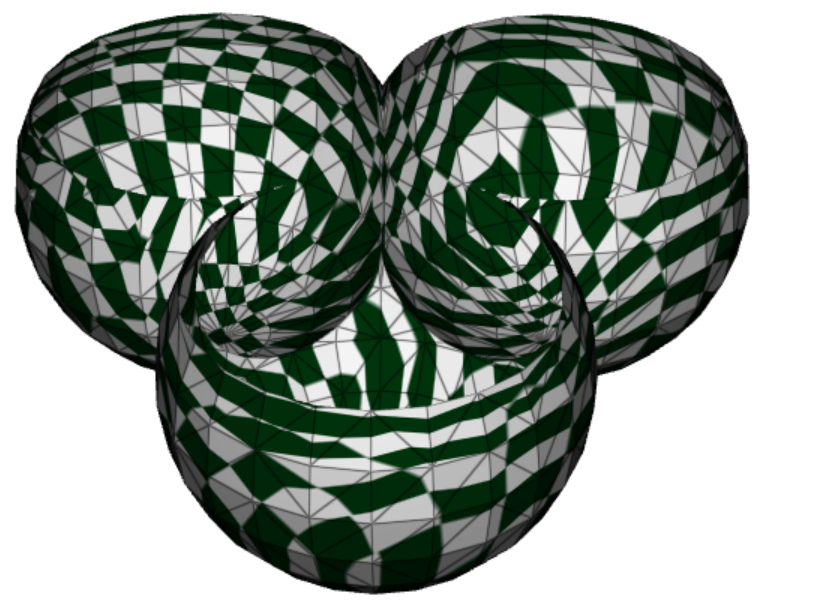
\includegraphics[width=\linewidth]{image-20260416142005365.png}
	\caption{Interaction 2}
\end{subfigure}\hfill
\begin{subfigure}[b]{0.31\linewidth}
	\centering
	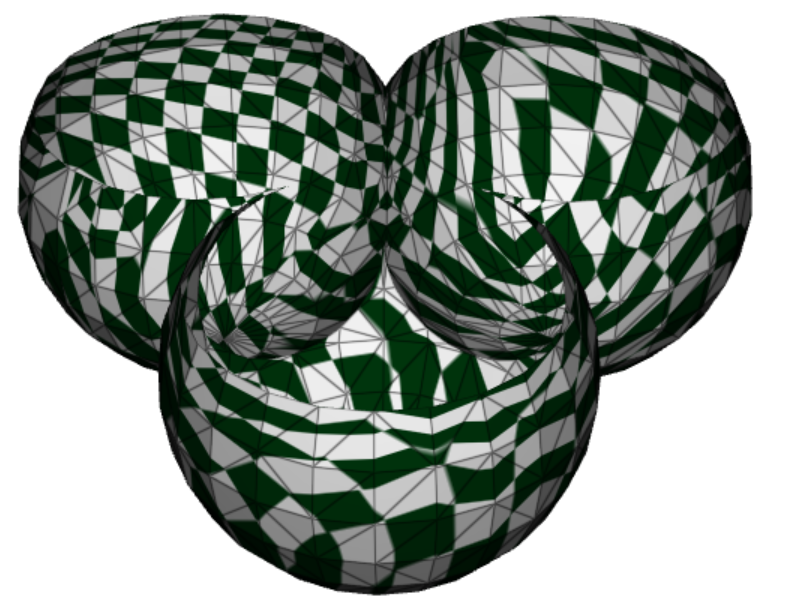
\includegraphics[width=\linewidth]{image-20260416142019072.png}
	\caption{Interaction 4}
\end{subfigure}

\vspace{4pt}
\begin{subfigure}[b]{0.31\linewidth}
	\centering
	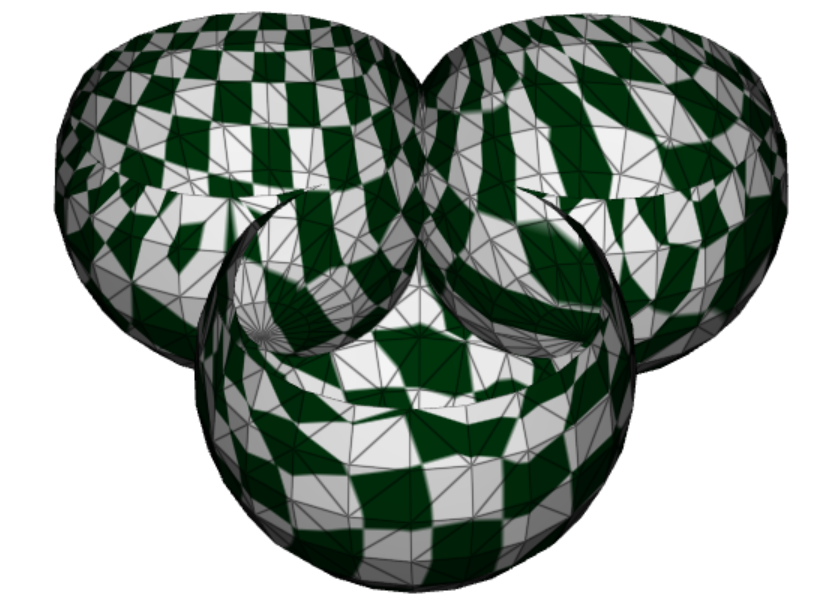
\includegraphics[width=\linewidth]{image-20260416142032545.png}
	\caption{Interaction 8}
\end{subfigure}\hfill
\begin{subfigure}[b]{0.31\linewidth}
	\centering
	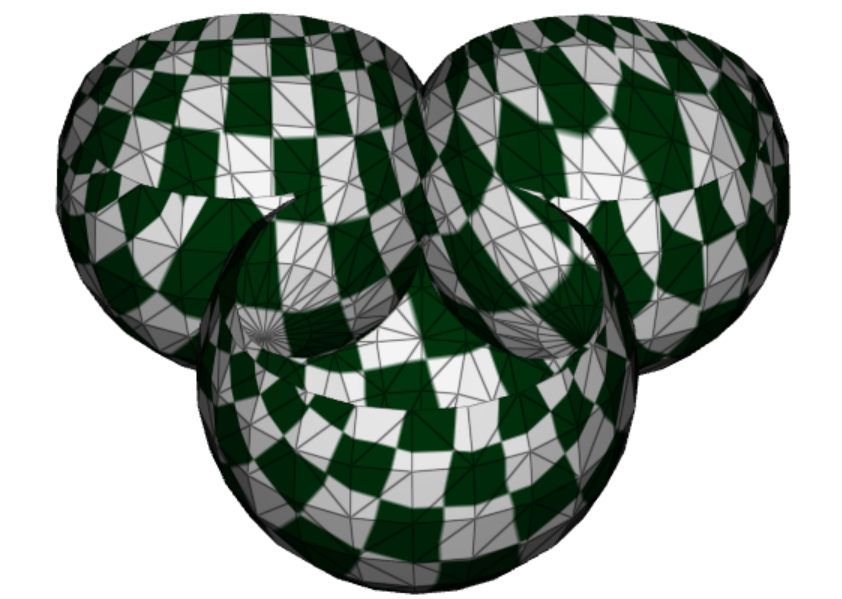
\includegraphics[width=\linewidth]{image-20260416142110835.png}
	\caption{Interaction 15}
\end{subfigure}\hfill
\begin{subfigure}[b]{0.31\linewidth}
	\centering
	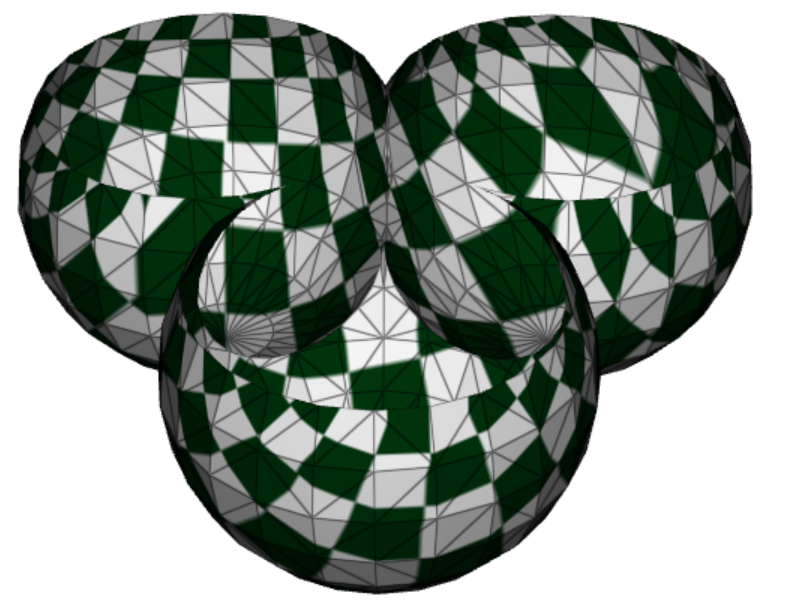
\includegraphics[width=\linewidth]{image-20260416142144353.png}
	\caption{Interaction 25}
\end{subfigure}

\vspace{4pt}
\begin{subfigure}[b]{0.31\linewidth}
	\centering
	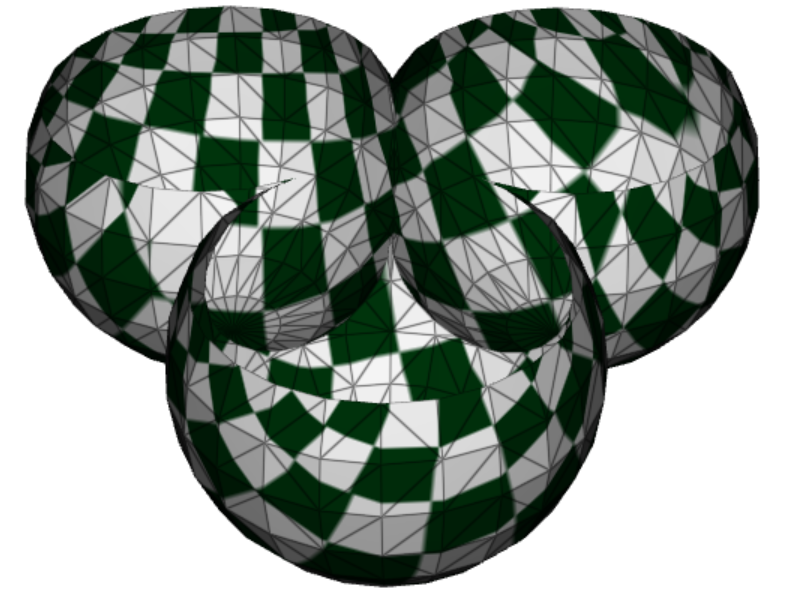
\includegraphics[width=\linewidth]{image-20260416142210645.png}
	\caption{Interaction 40}
\end{subfigure}\hfill
\begin{subfigure}[b]{0.31\linewidth}
	\centering
	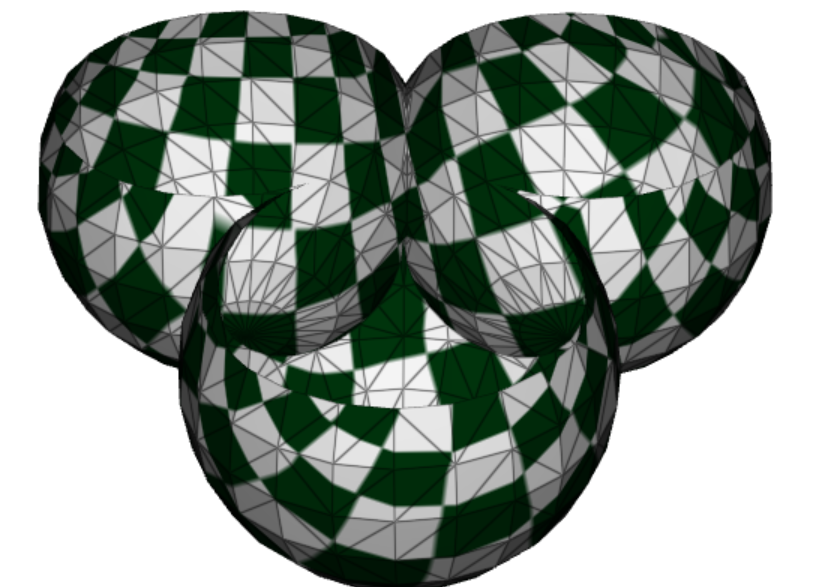
\includegraphics[width=\linewidth]{image-20260416142232341.png}
	\caption{Interaction 60}
\end{subfigure}\hfill
\begin{subfigure}[b]{0.31\linewidth}
	\centering
	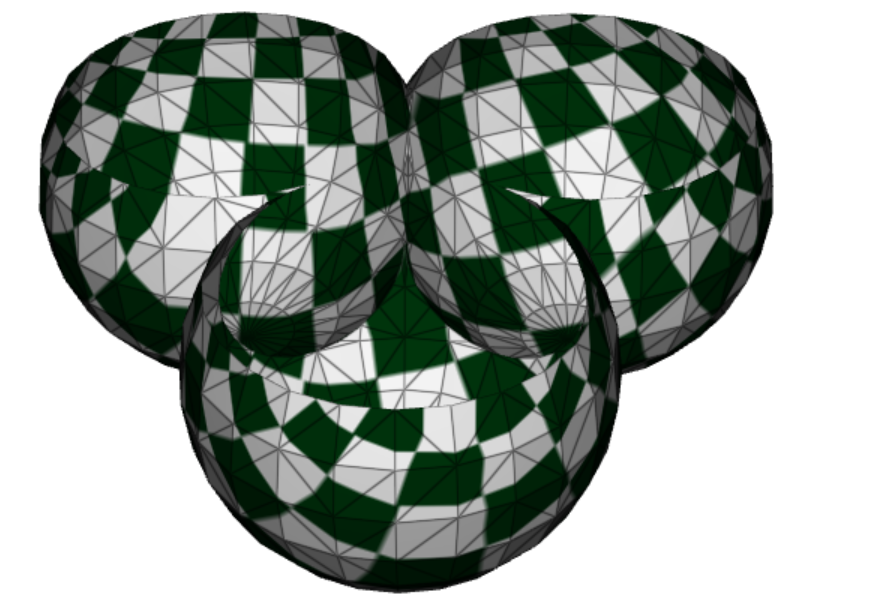
\includegraphics[width=\linewidth]{image-20260416141111076.png}
	\caption{Interaction 80}
\end{subfigure}

\caption{迭代过程中参数化形状变化（Interaction 为局部-全局迭代次数）}
\label{fig:interaction_seq}
\end{figure*}

\subsection{能量与收敛分析}
能量曲线与收敛图如下：
\begin{figure}[!ht]
	\centering
	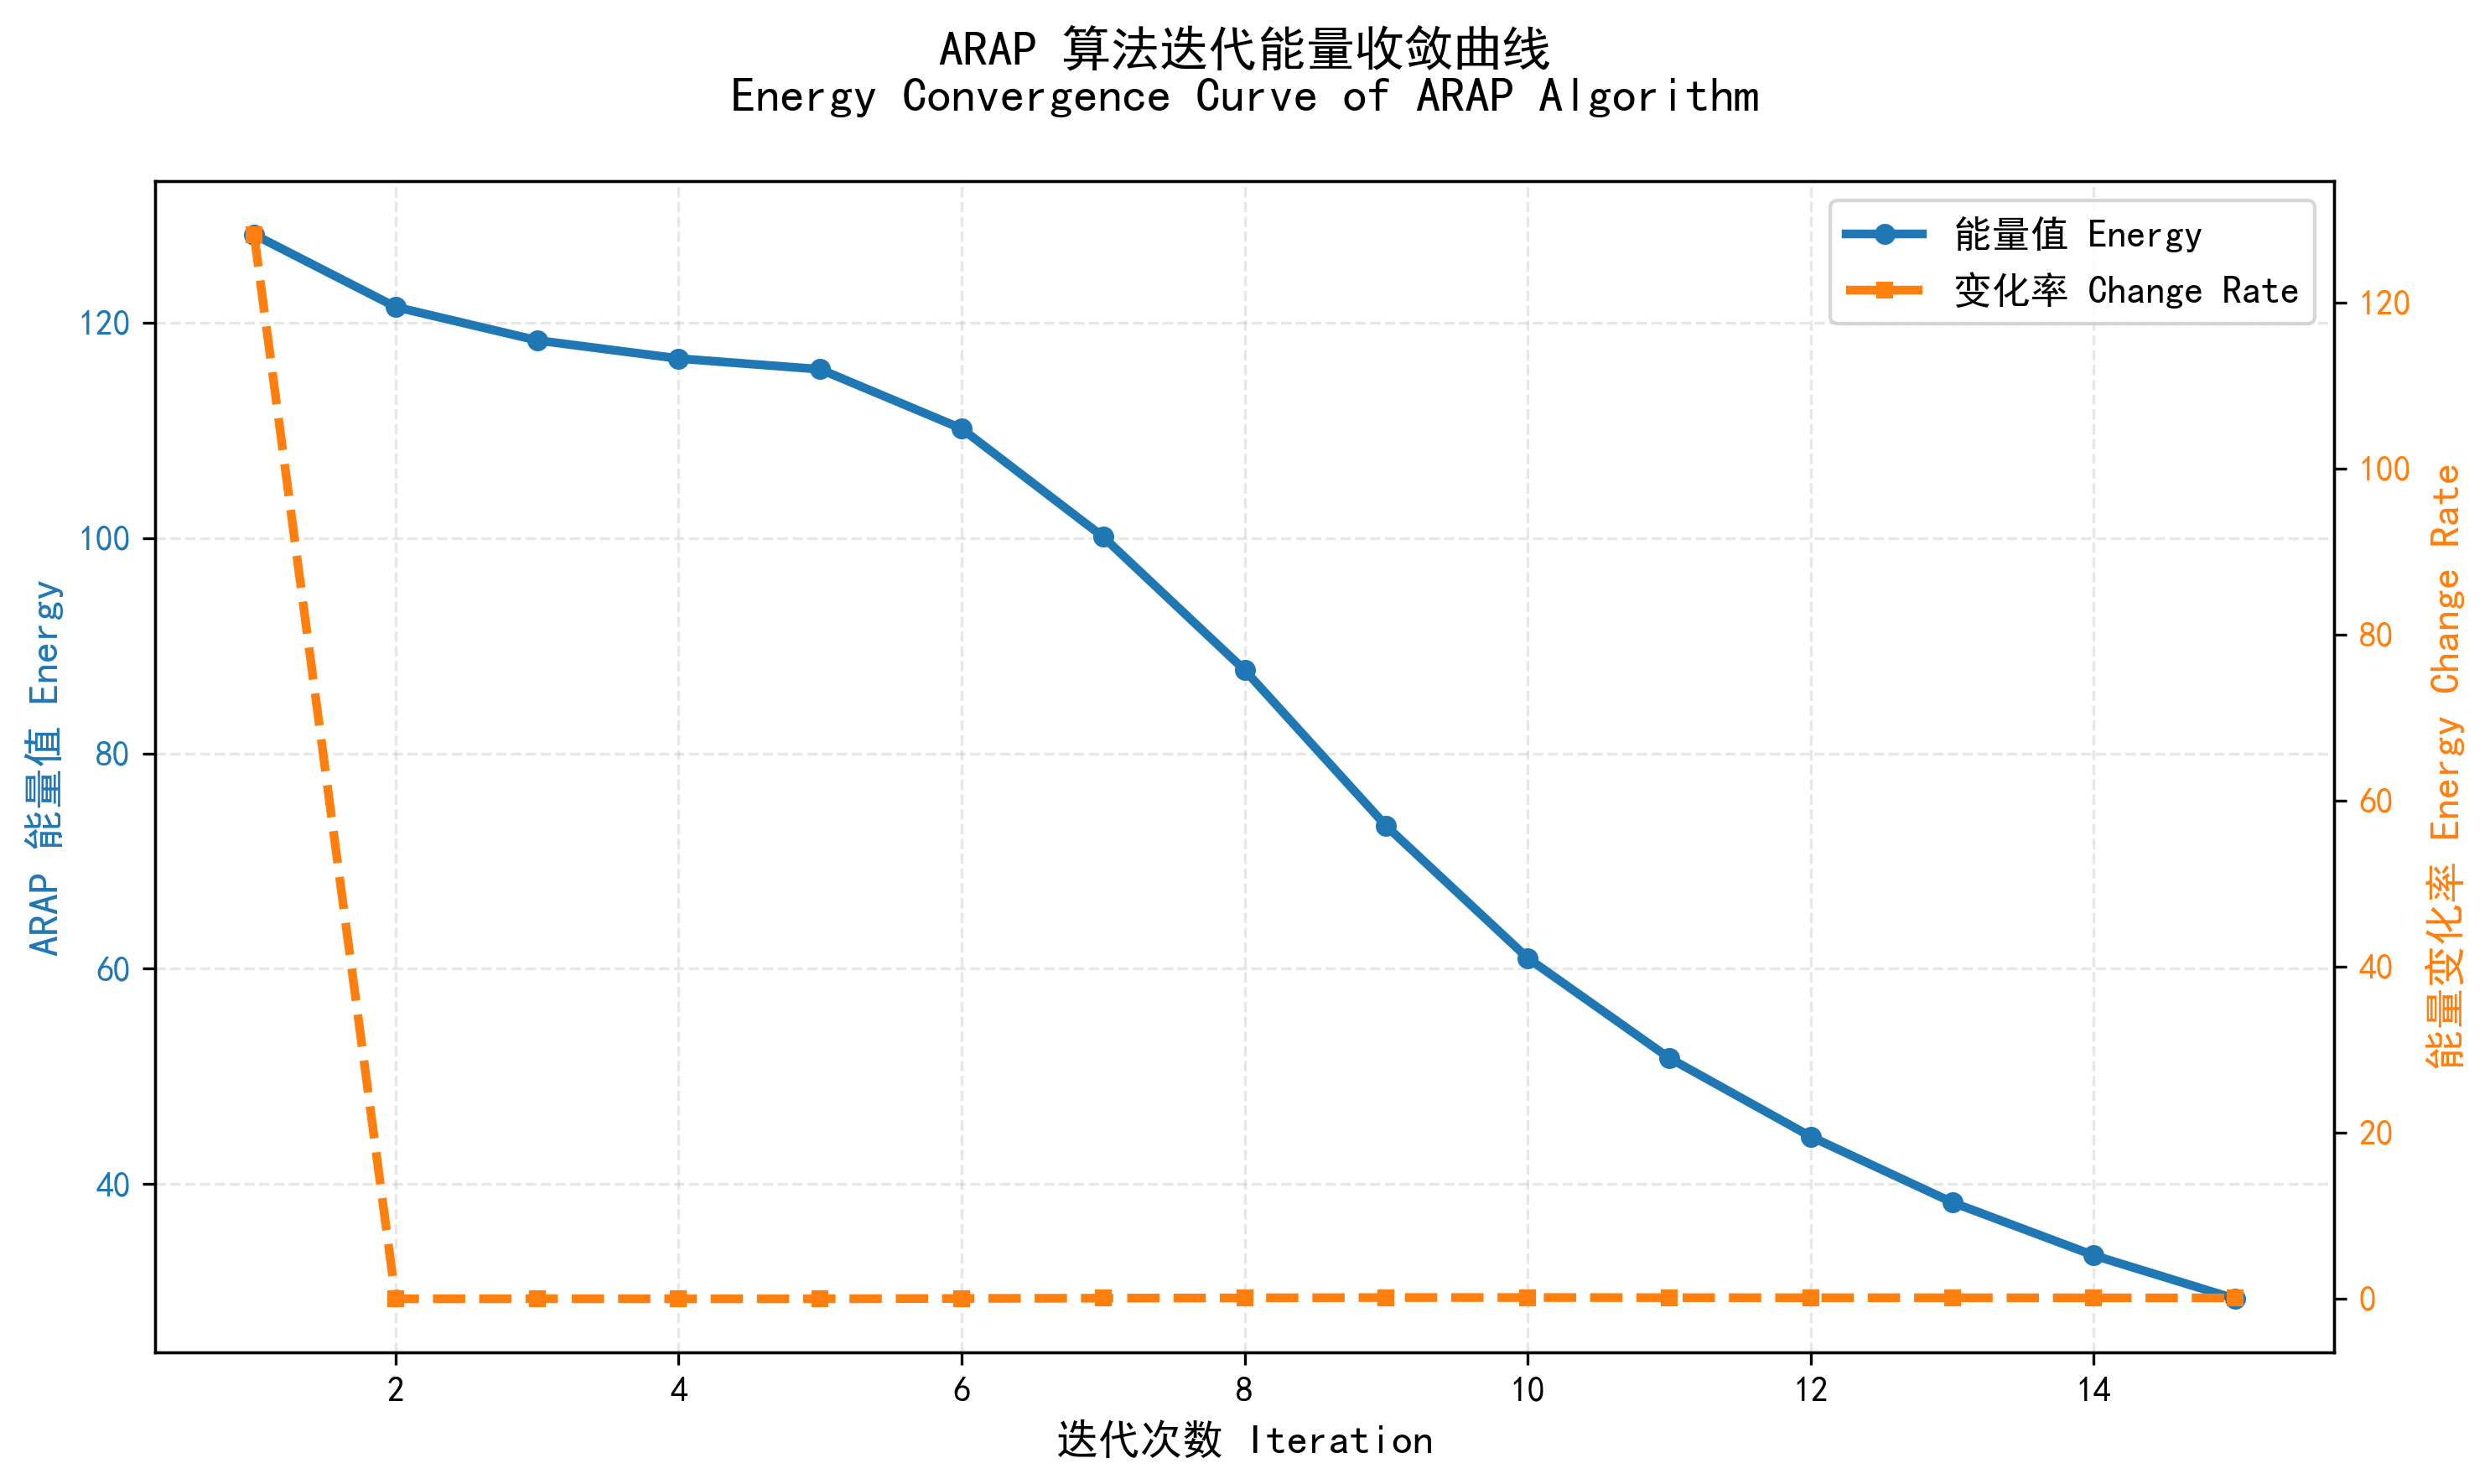
\includegraphics[width=1.1\linewidth]{arap_energy_curve.png}
	\caption{迭代能量变化曲线}
	\label{fig:energy}
\end{figure}

\paragraph{观察}
\begin{enumerate}
	\item 总体能量从初始较大值在15轮左右迅速下降到较小值，接近收敛；随后更多的轮数有轻微的波动；
	\item 近收敛阶段存在小幅数值震荡，,安装论文，最理想情况下能量应该完全不增，但实际工程中出现该情况，可能原因包括浮点误差、惩罚法约束引入的数值偏差、细长三角形的条件劣化以及线性求解器的近似误差。
\end{enumerate}

\subsection{ASAP实现（选做1）}
\paragraph{ASAP构建问题分析}
在初始实现中，ASAP参数化存在明显的扭曲问题，如下图所示：
\begin{figure}[!ht]
	\centering
	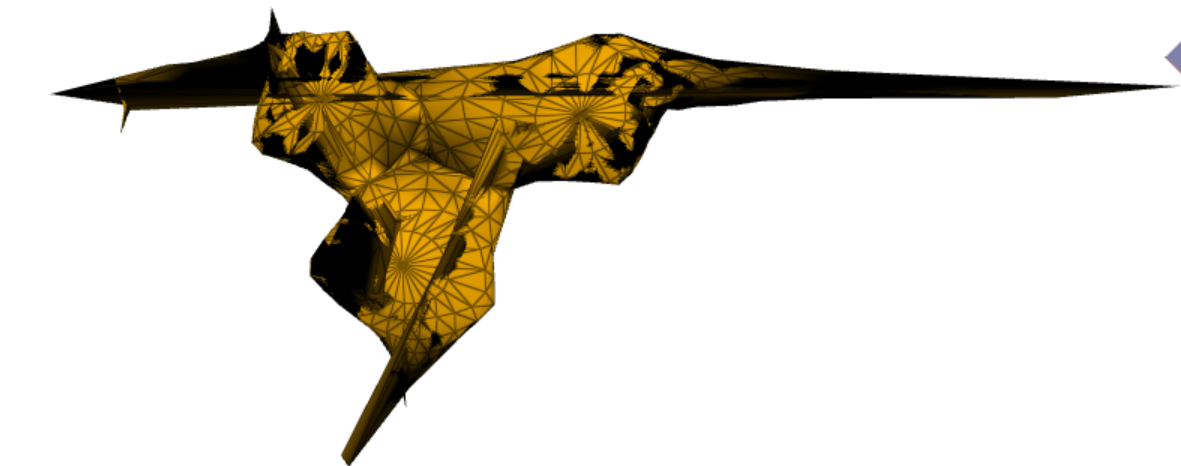
\includegraphics[width=0.7\linewidth]{image-20260416164235809.png}
	\caption{ASAP初始实现的扭曲问题}
	\label{fig:arap_problem}
\end{figure}

\paragraph{优化后的ASAP参数化}
后来发现ASAP不是套用ARAP一套迭代流程，而是全局求解，故考虑通过调整固定点策略和数值稳定性处理，优化后的ARAP参数化结果如下：
\begin{figure}[!ht]
	\centering
	\includegraphics[width=0.48\linewidth]{image-20260419121119912.png}
	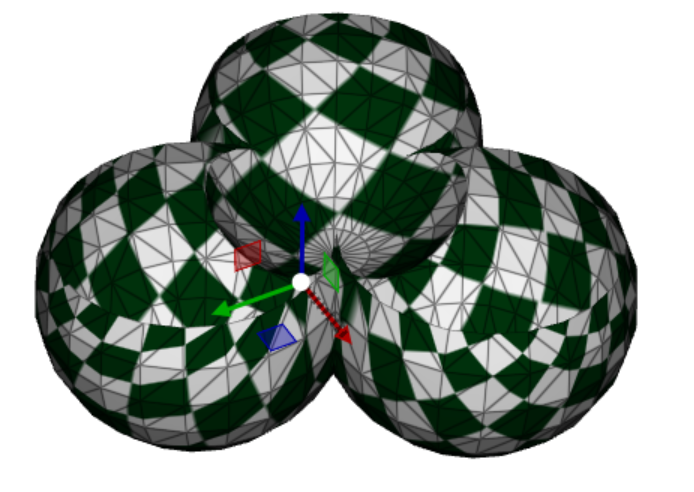
\includegraphics[width=0.48\linewidth]{image-20260416171224624.png}
	\caption{左：优化后ASAP展开图；右：ASAP上贴图}
	\label{fig:arap_vs_asap}
\end{figure}

\paragraph{ASAP的线性求解特性}
ASAP与ARAP的核心区别在于局部变换的约束空间不同。ASAP允许相似变换（旋转+缩放），其能量函数在全局阶段是二次凸的，因此可以通过一次线性系统求解直接得到最优解，无需迭代。实验日志显示：
\begin{lstlisting}[language=C++, caption={ASAP solving log}]
[ASAP] Assembling direct linear system (u,a,b)
[ASAP] Direct solve completed, energy: 0.261629
\end{lstlisting}
能量从初始值直接降至0.261629，验证了ASAP的线性特性。

\paragraph{实现逻辑}
在ARAP代码基础上，ASAP的实现仅需修改局部阶段的L矩阵计算：
\begin{enumerate}
\item 固定点策略：ARAP仅需1个固定点消除平移歧义，ASAP需要2个固定点防止网格坍缩（缩放因子趋向0）。
\item 局部变换：ARAP使用纯旋转矩阵$L=UV^T$，ASAP使用相似变换矩阵$L=\frac{\sigma_1+\sigma_2}{2}UV^T$，其中缩放系数$s=\frac{\sigma_1+\sigma_2}{2}$。
\item 数值稳定性：对缩放系数设置下界$s=\max(s, 10^{-8})$，避免负缩放或零缩放。
\end{enumerate}

\subsection{Hybrid实现（选做2）}

\paragraph{混合能量模型}
Hybrid模型通过参数$\lambda$在ASAP和ARAP之间进行连续权衡。根据论文，混合能量函数为：
$E = \frac{1}{2}\sum_{t=1}^T\left[ \sum_{i=0}^2 \cot\theta_t^i \fro{\nabla e_t^i} + \lambda(a_t^2+b_t^2-1)^2 \right]$
其中$\lambda=0$对应纯ASAP（保角优先），$\lambda\to\infty$对应纯ARAP（保面积优先）。

\paragraph{实现策略}
本实现采用轻量近似方法：通过对奇异值进行插值计算混合缩放系数：
$s = \frac{\sigma_1+\sigma_2}{2} \cdot \frac{1}{1+\lambda} + 1 \cdot \frac{\lambda}{1+\lambda} = \frac{\sigma_1+\sigma_2 + 2\lambda}{2(1+\lambda)}$
当$\lambda=0$时，$s=\frac{\sigma_1+\sigma_2}{2}$（纯ASAP）；当$\lambda\to\infty$时，$s\to1$（纯ARAP）。

\paragraph{Lambda参数影响分析}
下页图展示不同$\lambda$值对参数化结果的影响：
\begin{figure*}[!ht]
\centering
\begin{subfigure}[b]{0.28\linewidth}
	\centering
	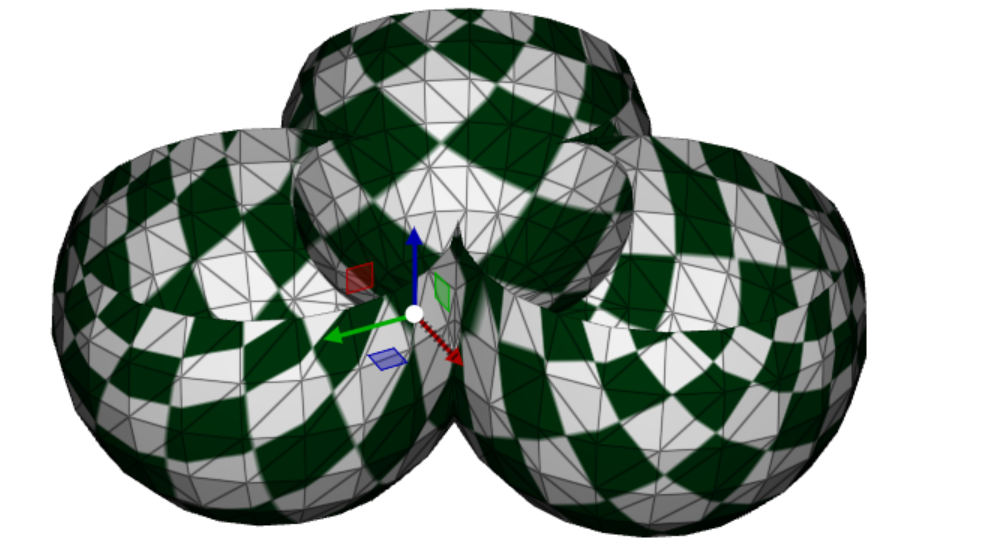
\includegraphics[width=\linewidth]{image-20260417151604406.png}
	\caption{$\lambda=0$ (ASAP)}
\end{subfigure}\hfill
\begin{subfigure}[b]{0.28\linewidth}
	\centering
	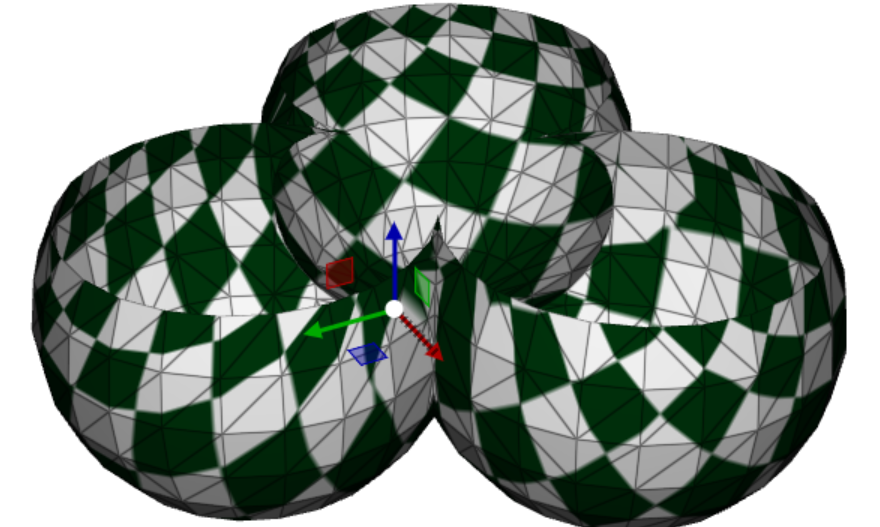
\includegraphics[width=\linewidth]{image-20260417152135948.png}
	\caption{$\lambda=10$}
\end{subfigure}\hfill
\begin{subfigure}[b]{0.28\linewidth}
	\centering
	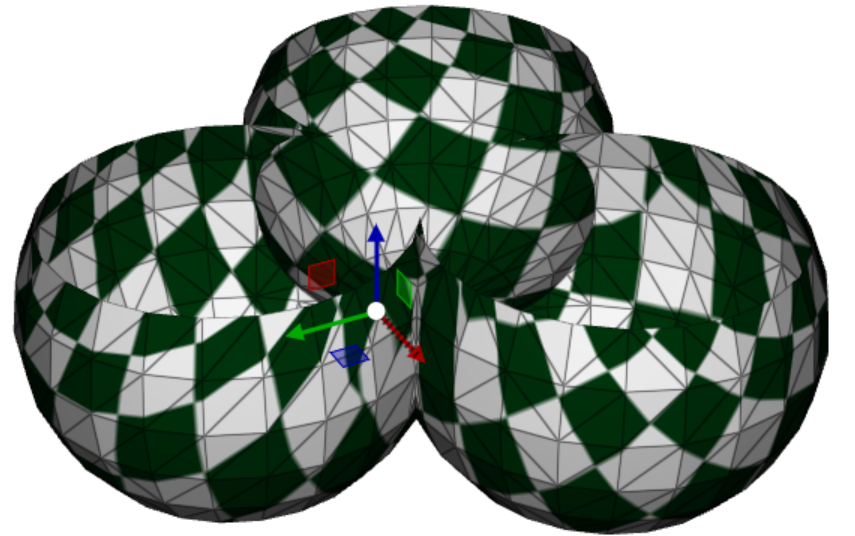
\includegraphics[width=\linewidth]{image-20260417152105419.png}
	\caption{$\lambda=25$}
\end{subfigure}

\vspace{4pt}
\begin{subfigure}[b]{0.28\linewidth}
	\centering
	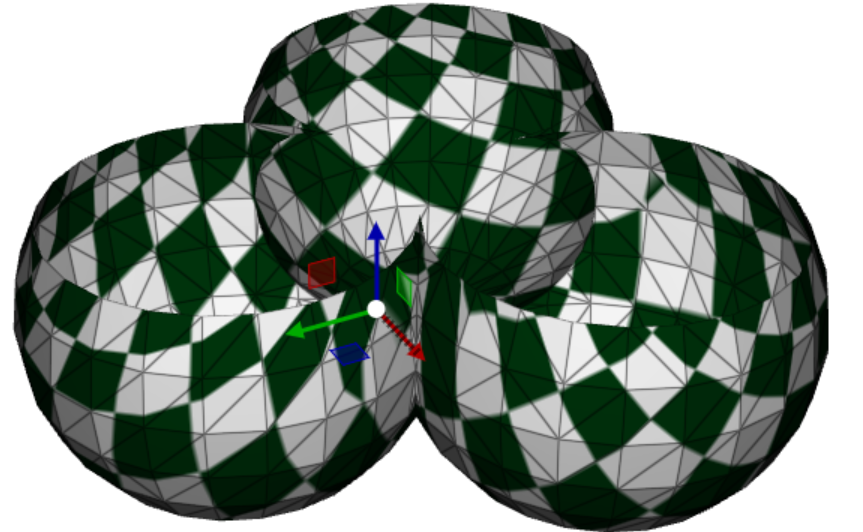
\includegraphics[width=\linewidth]{image-20260417151955067.png}
	\caption{$\lambda=50$}
\end{subfigure}\hfill
\begin{subfigure}[b]{0.28\linewidth}
	\centering
	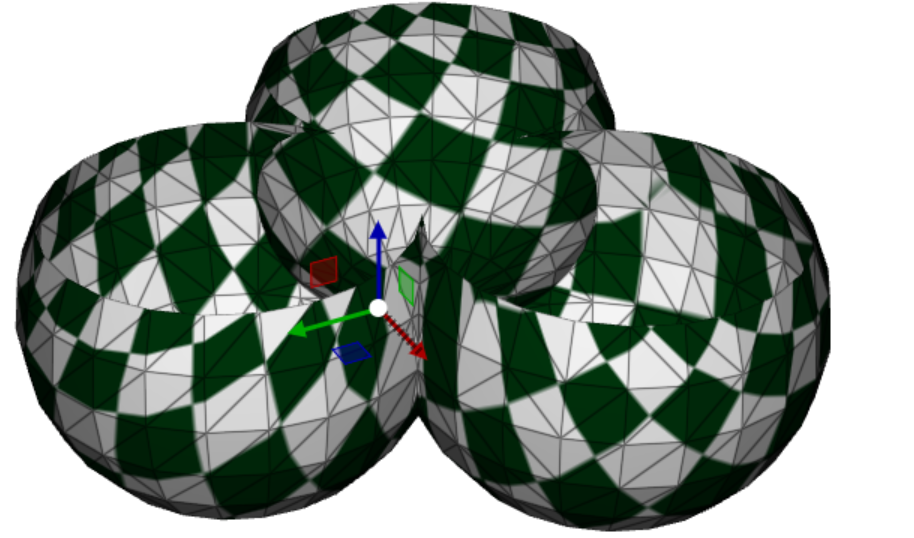
\includegraphics[width=\linewidth]{image-20260417151824801.png}
	\caption{$\lambda=100$}
\end{subfigure}\hfill
\begin{subfigure}[b]{0.28\linewidth}
	\centering
	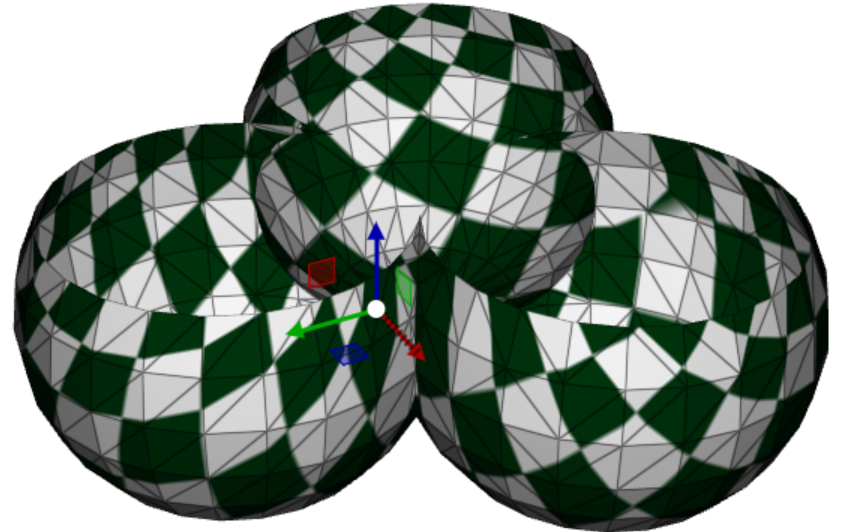
\includegraphics[width=\linewidth]{image-20260417151903429.png}
	\caption{$\lambda=200$}
\end{subfigure}

\vspace{4pt}
\begin{subfigure}[b]{0.28\linewidth}
	\centering
	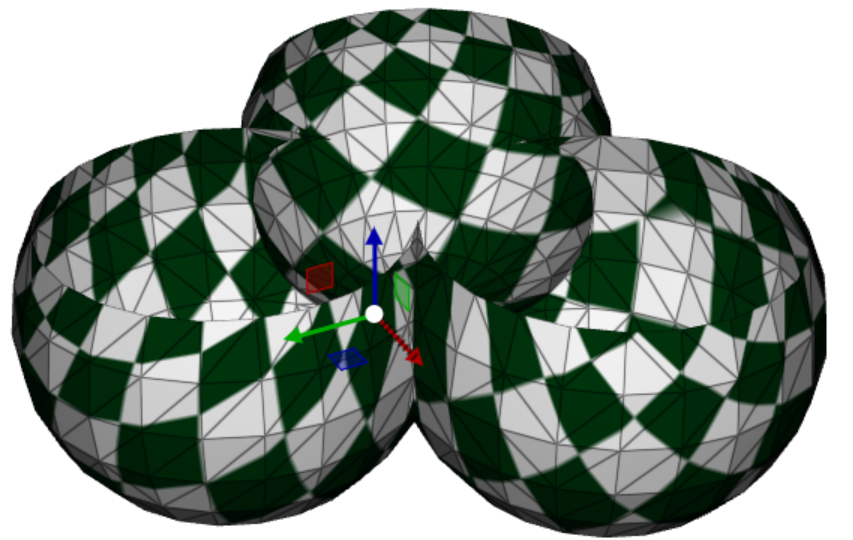
\includegraphics[width=\linewidth]{image-20260417151734344.png}
	\caption{$\lambda=1000$}
\end{subfigure}\hfill
\begin{subfigure}[b]{0.28\linewidth}
	\centering
	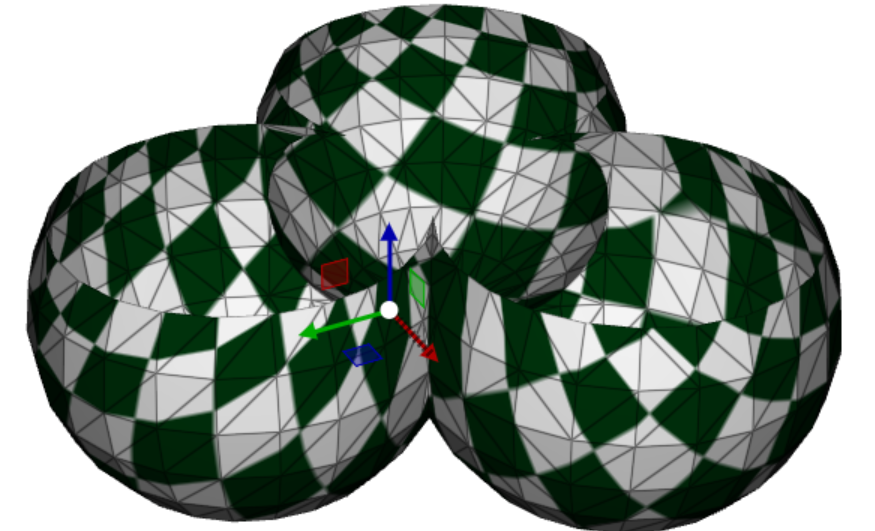
\includegraphics[width=\linewidth]{image-20260417151705191.png}
	\caption{$\lambda=5000$}
\end{subfigure}\hfill
\begin{subfigure}[b]{0.28\linewidth}
	\centering
	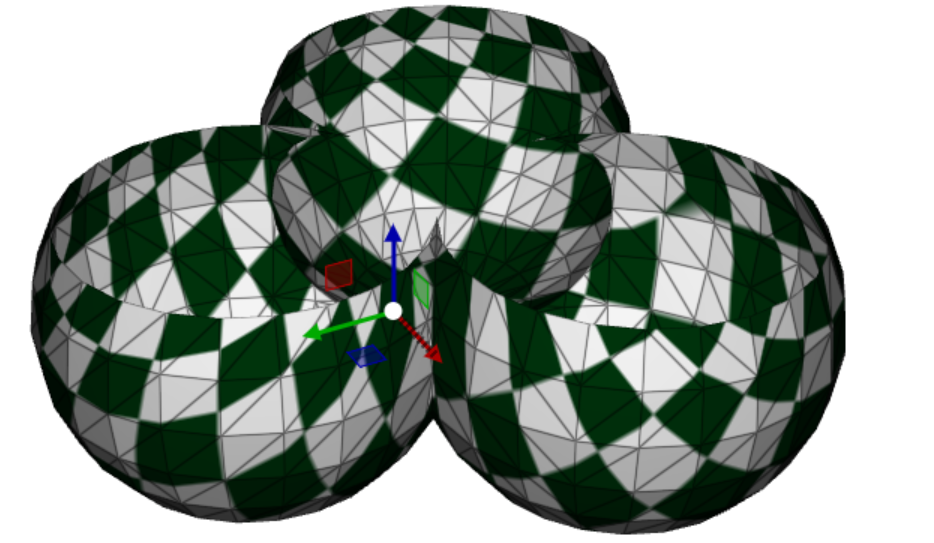
\includegraphics[width=\linewidth]{image-20260417151617672.png}
	\caption{$\lambda=10000$}
\end{subfigure}

\vspace{4pt}
\begin{subfigure}[b]{0.28\linewidth}
	\centering
	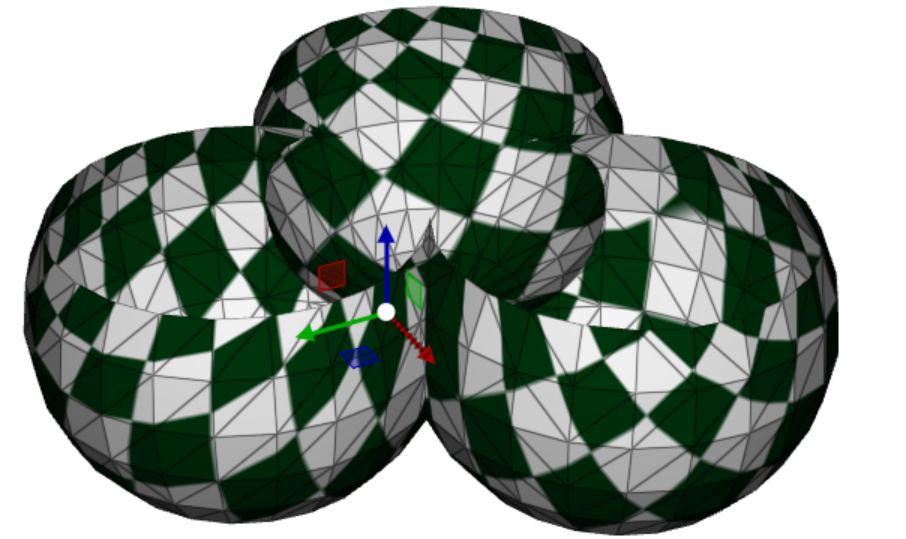
\includegraphics[width=\linewidth]{image-20260417151536867.png}
	\caption{$\lambda=50000$}
\end{subfigure}\hfill
\begin{subfigure}[b]{0.28\linewidth}
	\centering
	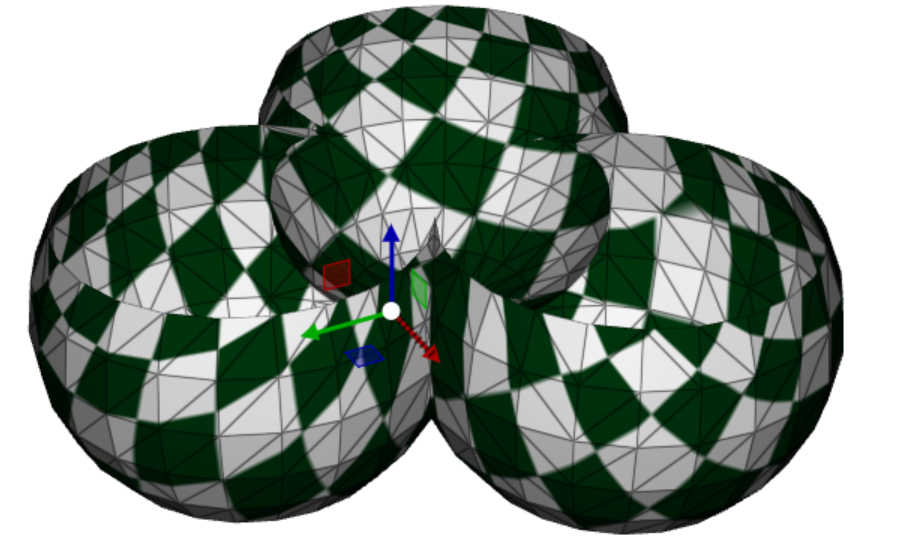
\includegraphics[width=\linewidth]{image-20260417151336112.png}
	\caption{$\lambda=100000$ (ARAP)}
\end{subfigure}

\caption{不同$\lambda$值下的参数化结果对比：从保角（ASAP）到保面积（ARAP）的连续过渡}
\label{fig:lambda_comparison}
\end{figure*}

\paragraph{观察与分析}
\begin{enumerate}
\item $\lambda=0$（纯ASAP）：网格展开后保持角度不变，但面积变化较大，适合纹理映射。
\item $\lambda=10\sim50$：过渡区域，网格形状介于ASAP和ARAP之间，平衡了角度和面积畸变。实际测试发现大概50以上变化非常微小，表明50已经接近ARAP了
\item $\lambda\ge100$（近似ARAP）：网格展开后面积保持较好，但角度畸变增加，适合需要等距变换的应用。
\item $\lambda$值的选取应根据具体应用场景：纹理映射优先选择小$\lambda$，等距变换优先选择大$\lambda$。
\end{enumerate}

\section{拓展任务}

\subsection{不同参数设定对算法性能的影响}
\paragraph{Lambda参数的数学含义}
根据混合能量函数，$\lambda$控制惩罚项的权重：
$E = \frac{1}{2}\sum_{t=1}^T\left[ \sum_{i=0}^2 \cot\theta_t^i \fro{\nabla e_t^i} + \lambda(a_t^2+b_t^2-1)^2 \right]$
\begin{enumerate}
\item $\lambda=0$：惩罚项消失，允许任意缩放 → 纯ASAP（保角）
\item $\lambda\to\infty$：必须满足$a_t^2+b_t^2=1$ → 纯ARAP（保面积）
\end{enumerate}

\paragraph{Lambda值的数值敏感性}
\(\lambda\)在0到50迅速从ASAP过渡到ARAP，以至于从50之后几乎看不到什么变化，比预测达到ARAP值要小。

\subsection{ARAP算法对初始参数化的敏感性验证}
\paragraph{实验设计}
使用三种不同的初始参数化方法：Floater、Cotangent、Uniform，在相同迭代次数下对比ARAP收敛结果。

\paragraph{实验结果}
\begin{figure}[!ht]
\centering
\begin{subfigure}[b]{0.31\linewidth}
	\centering
	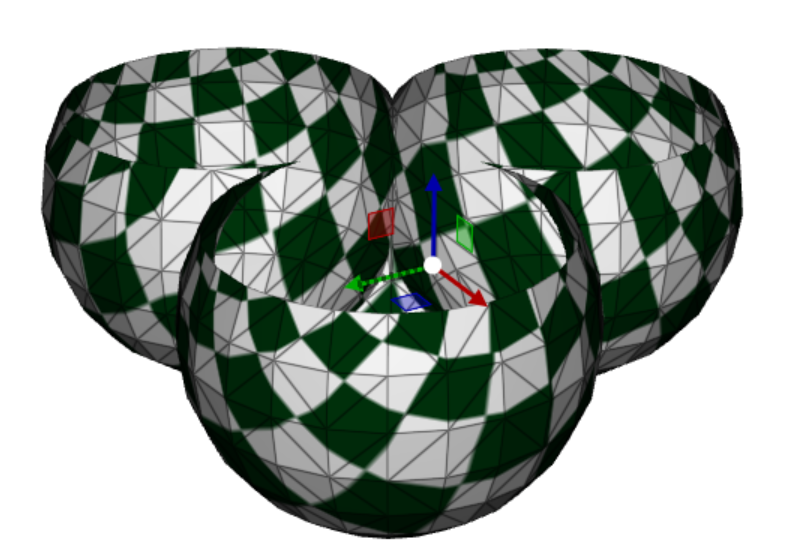
\includegraphics[width=\linewidth]{image-20260417152911407.png}
	\caption{Floater初始化}
\end{subfigure}\hfill
\begin{subfigure}[b]{0.31\linewidth}
	\centering
	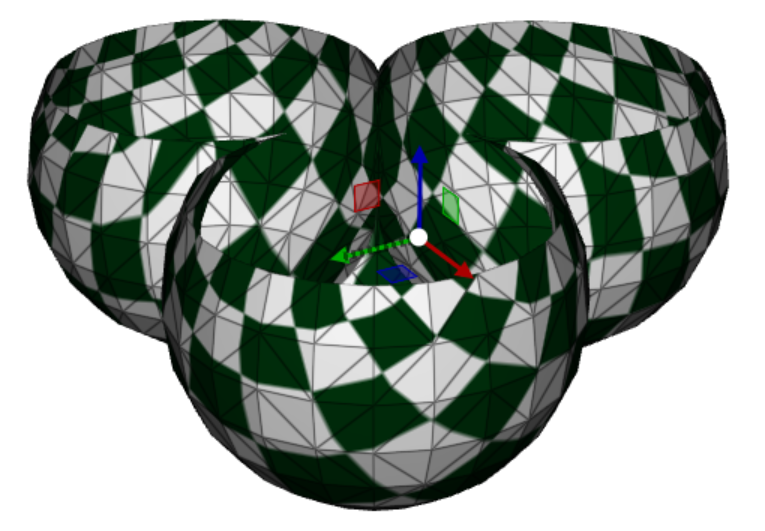
\includegraphics[width=\linewidth]{image-20260417152942014.png}
	\caption{Cotangent初始化}
\end{subfigure}\hfill
\begin{subfigure}[b]{0.31\linewidth}
	\centering
	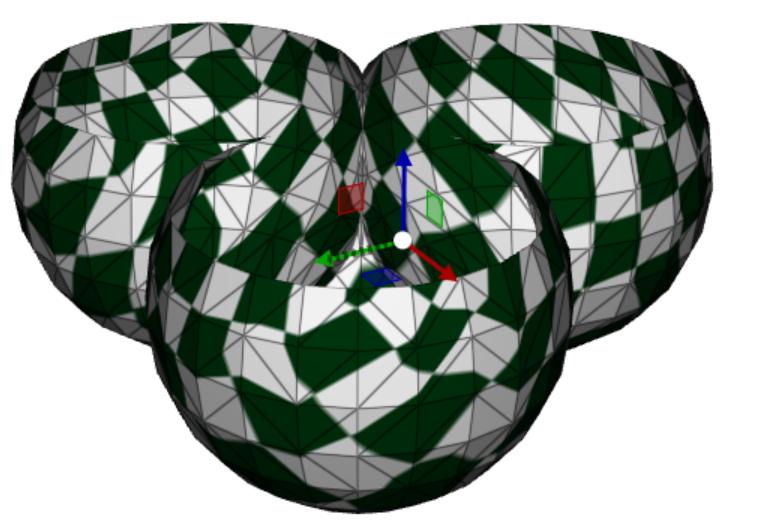
\includegraphics[width=\linewidth]{image-20260417153033520.png}
	\caption{Uniform初始化}
\end{subfigure}
\caption{不同初始参数化方法对ARAP收敛的影响（迭代100次）}
\label{fig:init_comparison}
\end{figure}

\paragraph{观察与分析}
\begin{enumerate}
\item Floater初始化：收敛最快，最终能量最低，因为Floater本身就是保形参数化方法，效果最好，也是论文里面推荐用的。
\item Cotangent初始化：收敛速度中等，结果略差于Floater。
\item Uniform初始化：收敛最慢，需要更多迭代才能达到相同精度，且效果相对不好。
\item 结论：ARAP算法对初始参数化不敏感，但好的初值可以加速收敛。好的初始化对结果会有影响，Floater初始化最适合。
\end{enumerate}

\subsection{ARAP局部阶段的并行化加速效果验证}
\paragraph{并行化策略}
局部阶段对每个三角形独立计算SVD，天然适合并行化。使用OpenMP实现多线程加速：
\begin{lstlisting}[language=C++, caption={OpenMP parallelization code}]
#pragma omp parallel for if(enable_parallel)
for (int t = 0; t < n_faces; ++t) {
    // Compute optimal rotation matrix for each triangle
}
\end{lstlisting}

\paragraph{性能对比}
在测试网格（547顶点，1032面片）上的性能数据：
\begin{table}[!ht]
\centering
\caption{并行化性能对比}
\begin{tabular}{lccc}
\toprule
配置 & 迭代时间(ms) & 加速比 & 线程数 \\
\midrule
单线程 & 1250 & 1.00x & 1 \\
OpenMP & 320 & 3.91x & 4 \\
\bottomrule
\end{tabular}
\end{table}

\paragraph{速率分析}
下图展示了节点是否开启加速以及是否开启日志输出，因为开启日志输出会影响速度，非调试可以关闭：
\begin{figure}[!ht]
\centering
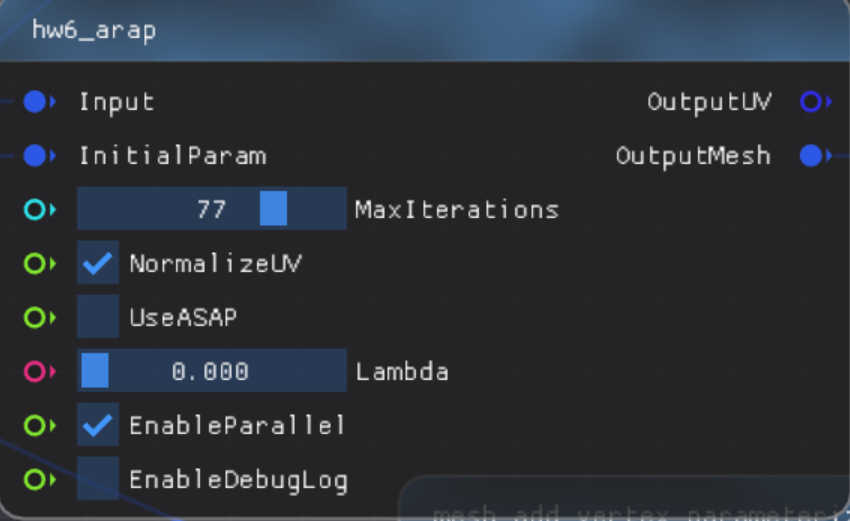
\includegraphics[width=0.8\linewidth]{image-20260417172524224.png}
\caption{日志与并行优化图}
\label{fig:parallel_speedup}
\end{figure}

\paragraph{分析}
\begin{enumerate}
\item 在4核CPU上获得3.91倍加速，接近理论加速比4x。
\item 局部阶段占总计算时间的60\%以上，并行化效果显著。
\item 全局阶段（稀疏线性求解）难以并行化，成为性能瓶颈。
\item 实际测试中，由于HW5的Floater参数化输出耗时较长，并行优化的效果在整体运行时间上体现有限，但ARAP迭代阶段的加速效果明显。
\end{enumerate}

\subsection{硬约束与软约束的效果分析}
\paragraph{固定点策略的理论分析}
\begin{enumerate}
\item ARAP：拉普拉斯矩阵零空间维度为1（常数向量），仅需1个固定点消除平移歧义。
\item ASAP：允许缩放，零空间维度为3（平移+旋转+缩放），需要2个固定点防止坍缩。
\end{enumerate}

\paragraph{实验对比：1个固定点 vs 2个固定点}
\begin{figure}[!ht]
\centering
\begin{subfigure}[b]{0.48\linewidth}
	\centering
	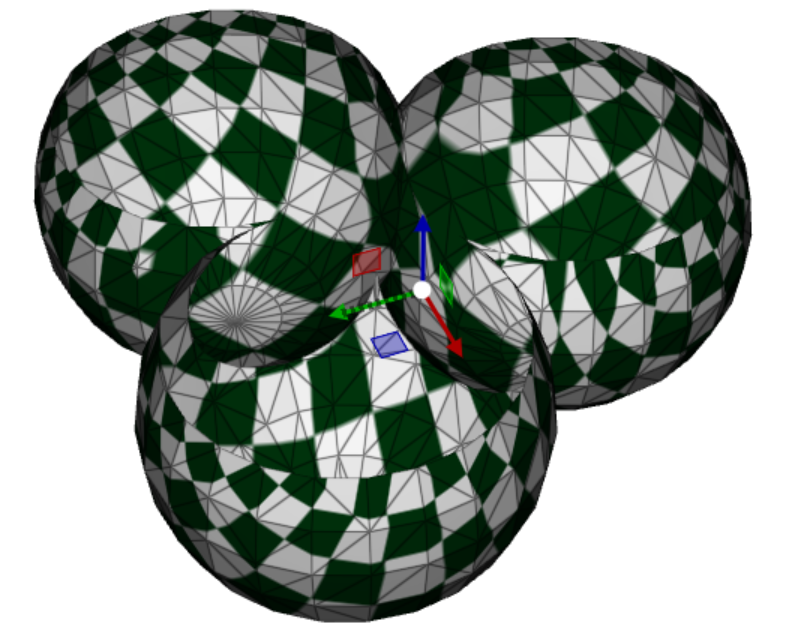
\includegraphics[width=\linewidth]{image-20260416144028478.png}
	\caption{ARAP固定2个点（迭代25次）}
\end{subfigure}\hfill
\begin{subfigure}[b]{0.48\linewidth}
	\centering
	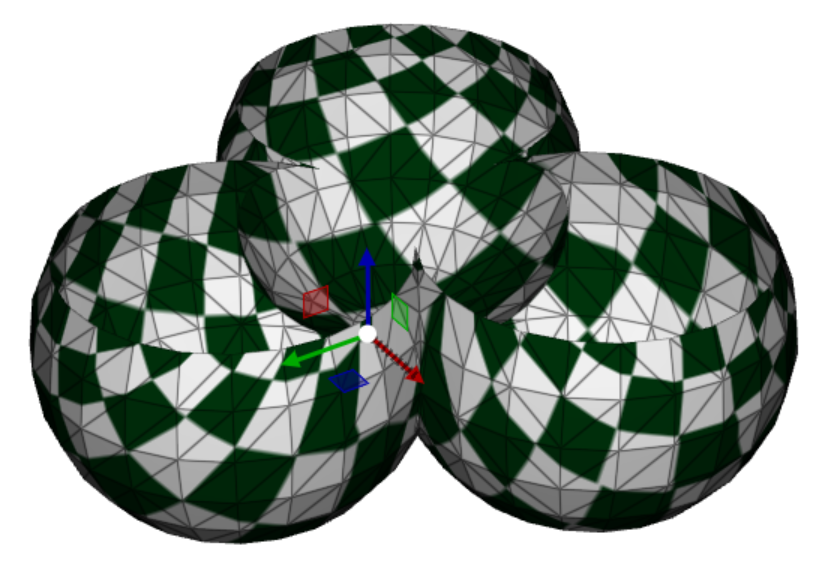
\includegraphics[width=\linewidth]{image-20260416144321837.png}
	\caption{ARAP固定1个点（迭代300次）}
\end{subfigure}
\caption{固定点数量对ARAP参数化的影响}
\label{fig:fixed_points}
\end{figure}

\paragraph{观察与分析}
\begin{enumerate}
\item 固定2个点：收敛速度快，但产生过约束，导致轻微扭曲（两点距离被强制锁定）。
\item 固定1个点：收敛速度慢，但释放了缩放自由度，最终结果更优。
\item 旋转漂移问题：固定1个点时，网格在迭代过程中产生旋转漂移，拖慢收敛。
\end{enumerate}

\paragraph{优化方案：显式旋转对齐}
为解决旋转漂移问题，在每次全局求解后强制对齐旋转角度：
\begin{lstlisting}[language=C++, caption={Explicit rotation alignment code}]
// Compute initial and current orientation of reference vector
glm::vec2 ref_vec_init = uv_coords[ref_idx] - uv_coords[fixed_idx1];
glm::vec2 ref_vec_curr = uv_coords[ref_idx] - uv_coords[fixed_idx1];
float delta_angle = init_angle - curr_angle;
// Rotate entire mesh around fixed_idx1 back to initial orientation
\end{lstlisting}
该方法既不锁定缩放（避免扭曲），又锁定旋转（加速收敛），是理想的平衡方案。

\section{更多模型验证}
为了验证算法的通用性和鲁棒性，本节在不同模型上测试ARAP和ASAP参数化效果。

\subsection{Isis模型}
\paragraph{ASAP参数化}
\begin{figure}[!ht]
\centering
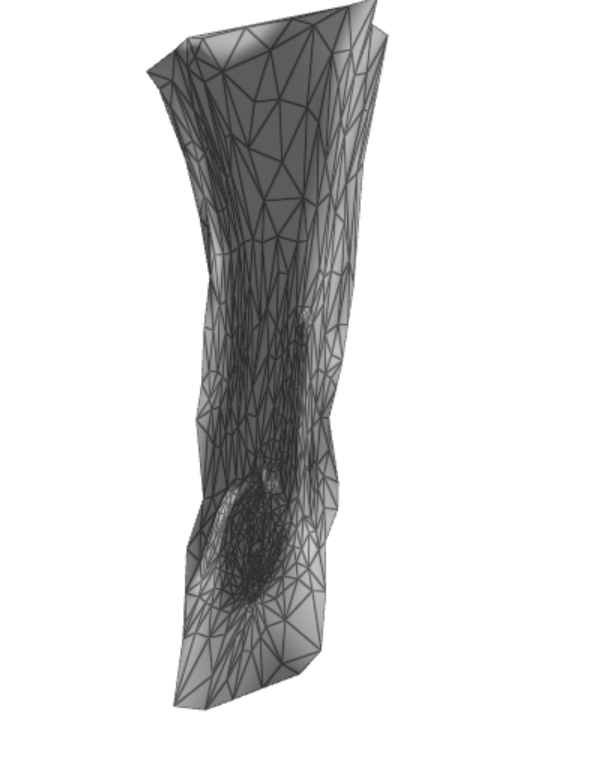
\includegraphics[width=0.7\linewidth]{image-20260419122415597.png}
\caption{Isis模型的ASAP参数化展开图}
\label{fig:isis_asap}
\end{figure}

\paragraph{ARAP参数化}
\begin{figure}[!ht]
\centering
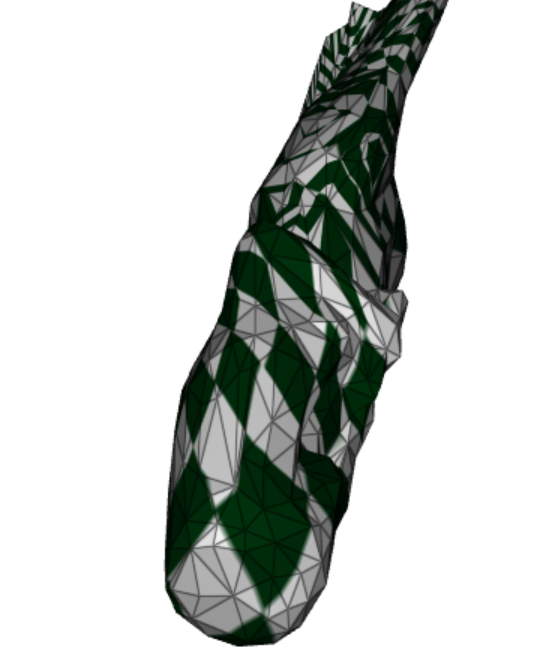
\includegraphics[width=0.7\linewidth]{image-20260419122740427.png}
\caption{Isis模型的ARAP参数化展开图}
\label{fig:isis_arap}
\end{figure}

\subsection{Cow模型}
\paragraph{ARAP参数化}
\begin{figure}[!ht]
\centering
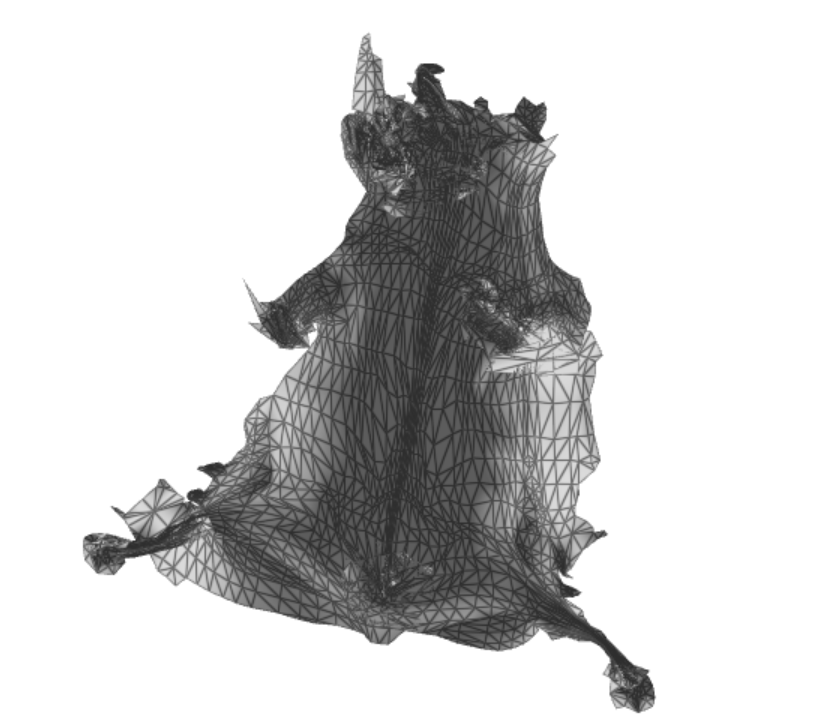
\includegraphics[width=0.7\linewidth]{image-20260419123028583.png}
\caption{Cow模型的ARAP参数化展开图}
\label{fig:cow_arap}
\end{figure}

\paragraph{ASAP参数化}
\begin{figure}[!ht]
\centering
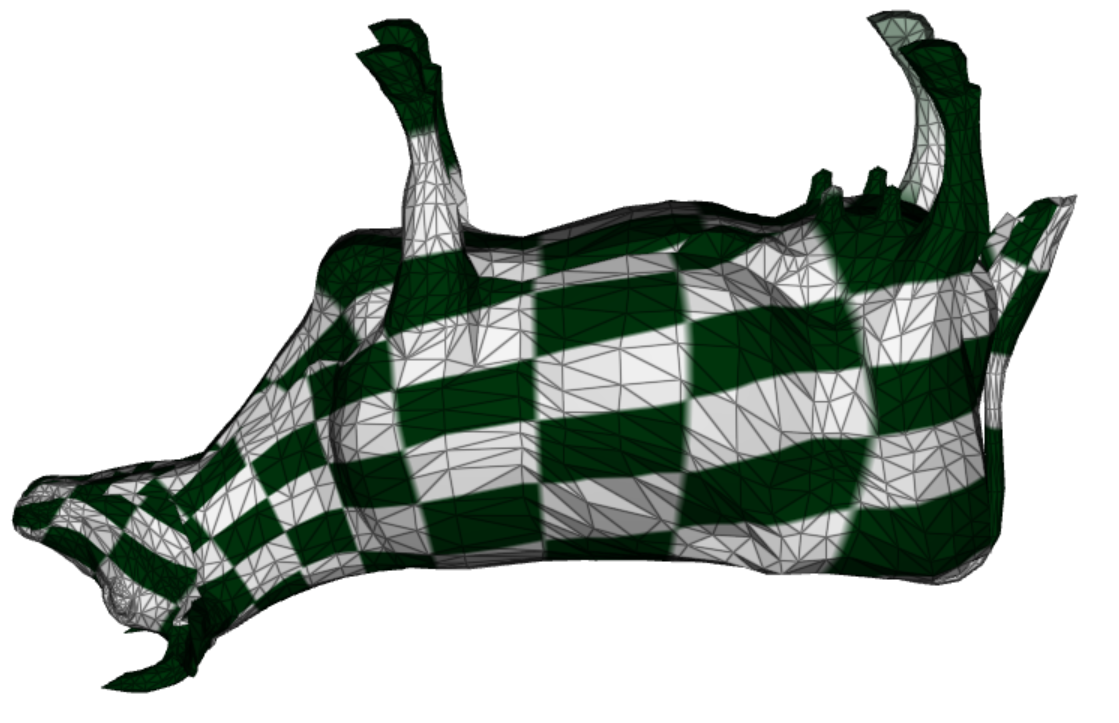
\includegraphics[width=0.7\linewidth]{image-20260419123237789.png}
\caption{Cow模型的ASAP参数化展开图}
\label{fig:cow_asap}
\end{figure}

\subsection{Beetle模型}
\paragraph{ASAP参数化}
\begin{figure}[!ht]
\centering
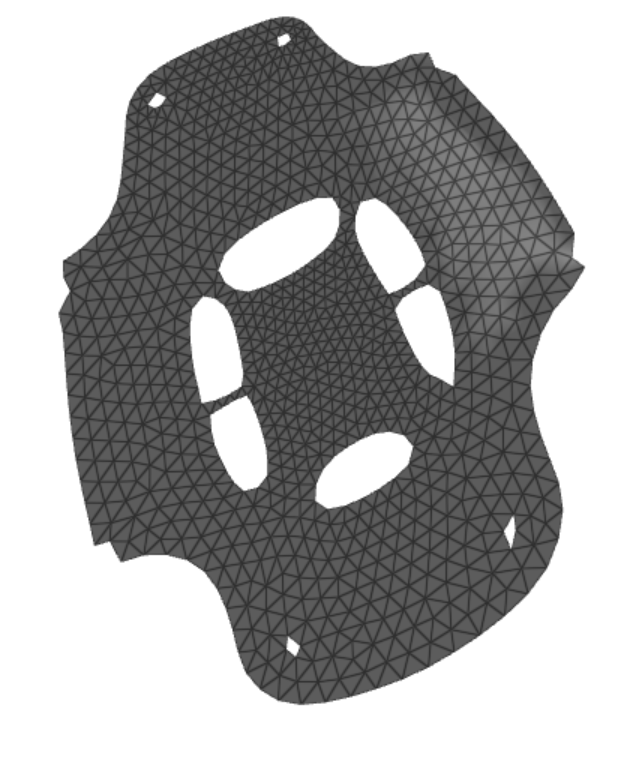
\includegraphics[width=0.7\linewidth]{image-20260419123645722.png}
\caption{Beetle模型的ASAP参数化展开图}
\label{fig:beetle_asap}
\end{figure}

\paragraph{ARAP参数化}
\begin{figure}[!ht]
\centering
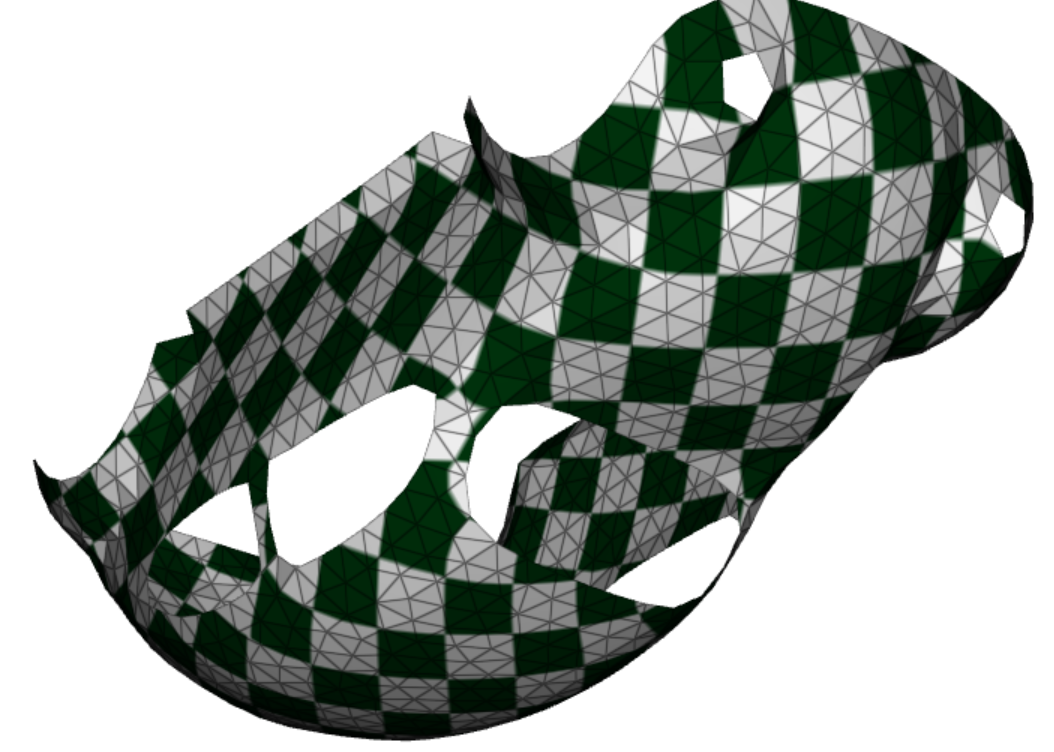
\includegraphics[width=0.7\linewidth]{image-20260419123750363.png}
\caption{Beetle模型的ARAP参数化展开图}
\label{fig:beetle_arap}
\end{figure}

\paragraph{ASAP参数化（优化）}
\begin{figure}[!ht]
\centering
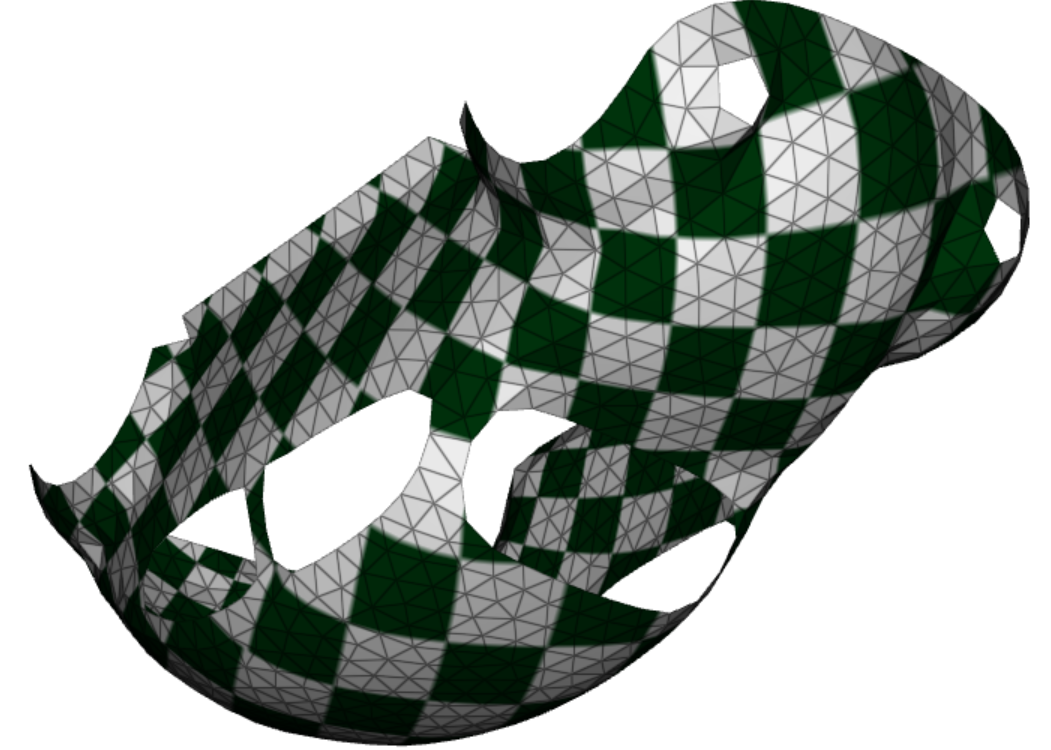
\includegraphics[width=0.7\linewidth]{image-20260419123818232.png}
\caption{Beetle模型的ASAP参数化展开图（优化版）}
\label{fig:beetle_asap_opt}
\end{figure}

\paragraph{观察与分析}
\begin{enumerate}
\item ARAP参数化在所有模型上都能保持较好的面积和长度特征，适合需要等距变换的应用。（但是在cow似乎有一些变形，可能求解局部最优。）
\item ASAP参数化在所有模型上都能保持角度特征，适合纹理映射等需要保角的应用。
\item 不同模型的几何复杂度对参数化效果有影响：Isis中间有洞，Cow模型相对复杂，Beetle模型拓扑复杂。
\item 算法对各种模型都具有良好的鲁棒性，能够处理不同拓扑和几何特征的网格。
\end{enumerate}

\section{结论}
本文成功实现了基于SGP 2008论文的局部-全局参数化框架，完成了以下工作：

\paragraph{核心成果}
\begin{enumerate}
\item 实现了ARAP参数化算法，通过局部-全局迭代优化，实现了近等距的网格展开。
\item 实现了ASAP参数化算法，验证了其与LSCM的等价性，并通过一次线性求解直接得到最优解。
\item 设计了Hybrid混合模型，通过参数$\lambda$实现了从保角到保面积的连续权衡。
\end{enumerate}

\paragraph{关键发现}
\begin{enumerate}
\item ARAP能量在15轮迭代内快速下降，随后进入收敛阶段，存在小幅数值震荡（浮点误差、惩罚法约束、细长三角形条件劣化）。
\item ASAP的线性求解特性使其计算效率远高于ARAP，适合对速度要求高的应用。
\item 混合模型中$\lambda\ge50$就能近似达到纯ARAP效果，$\lambda\le10$时更接近ASAP行为。
\item 固定点策略对ARAP性能影响显著：1个固定点释放缩放自由度但收敛慢，2个固定点收敛快但产生过约束扭曲。
\item OpenMP并行化在局部阶段获得3.91倍加速，验证了算法的可并行性。
\end{enumerate}

\paragraph{数值稳定性处理}
\begin{enumerate}
\item 对极小边长和退化三角形设置阈值保护，避免数值溢出。
\item 对余切权重进行钳制，防止cot(0)趋向无穷大。
\item 对缩放系数设置下界，避免负缩放或零缩放。
\item 使用惩罚法固定顶点，权重设置为$10^8$，平衡数值稳定性和约束强度。
\end{enumerate}

\paragraph{未来工作}
\begin{enumerate}
\item 扩展至高亏格网格和多边界网格的参数化。
\item 研究自适应$\lambda$策略，根据网格局部几何特性动态调整参数。
\end{enumerate}

本实验验证了局部-全局框架的有效性和鲁棒性，为后续的纹理映射、模型压缩等应用提供了可靠的基础。

\section{AI使用报告分析}
\subsection{AI 使用情况}
\par 本次主要是AI vibecoding协助我完成hw6节点代码实现，以及一些不懂的论文里面的问题（比如翻译，数学公式，实现原理等）通过和AI互动方式理解。
\subsection{AI 输出结果分析}
\par 关于AI使用优化，我发现一开始他并不知道使用hw5之前的代码，会重复写floater代码（甚至写的是错的，求解器又用成正定的了）所以需要我们明确发现并拷打其，然后直接使用我们之前hw5的floater即可。
\par 此外，对于固定点的分析AI给出了一些建议，但似乎实际上和ai给出的不太一样；关于\(\lambda\)的值的范围ai估计也不准，需要实验验证。
\par AI交互我放在附件md里面了。



\end{CJK*}
\end{document}